\begin{frame}
\frametitle{Quantum information is \emph{different}}
\begin{itemize}
  \item \textbf{Quantum simulation}
  \begin{itemize}
    \item Classical: $\ket{00101101\ldots}$ - $N$ bits of information.
    \item Quantum: $c_1 \ket{\ldots 001} + c_2 \ket{\ldots 010} + \cdots$ - $2^N$ coefficients.
  Run out of memory!
  \end{itemize}
  \pause
  \item \textbf{Computation}
  \begin{figure}
  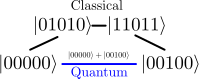
\includegraphics[scale=0.8]{classical_vs_quantum_paths.pdf}
  \end{figure}
  Quantum ``trajectories'' are more rich.
  \begin{itemize}
    \item Grover's algorithm: invert a function in $\sqrt{N}$ time instead of $N$.
    \item Shor's algorithm: factor a number in $\text{Polynomial}(b)$ instead of $\exp\left( (1.9 + o(1))(b \ln 2)^{1/3} ( \ln(b \ln 2))^{2/3} \right)$.
  \end{itemize}
  \pause
  \item Yet quantum information is terrible for e.g. basic arithmetic.
\end{itemize}
\end{frame}
